\documentclass{article}

\usepackage[utf8]{inputenc}
\usepackage[T1]{fontenc}
\usepackage{fancyvrb}

\usepackage{Sweave}
\begin{document}
\Sconcordance{concordance:adaline.tex:adaline.Rnw:%
1 6 1 1 0 18 1 1 3 1 0 1 2 2 1 1 2 3 1 5 0 1 3 4 1 1 2 1 0 2 2 3 1 2 2 %
3 1 3 0 1 2 4 1 1 2 1 0 1 1 1 2 1 0 1 2 1 1 6 0 1 2 4 1 1 2 1 0 1 2 3 1 %
4 0 1 2 4 1 1 2 9 0 1 2 8 1 1 2 1 0 1 2 2 1 1 2 2 1 1 2 4 1 4 0 1 2 4 1 %
1 2 1 0 1 1 1 2 5 1 3 2 4 1 1 2 3 0 1 2 4 1 1 2 1 0 1 1 1 2 1 0 1 2 1 1 %
6 0 1 2 4 1 1 2 1 0 1 2 4 1 4 0 1 2 4 1 1 2 11 0 1 2}


\title{Treinamento do Adaline}
\author{Matheus Araujo - 2013066265}
\date{}

\maketitle

O objetivo da atividade dessa semana é compreender melhor o funcionamento do método \emph{Adaline} através dos dois exercícios apresentados a seguir.

\section{Exercício 1}

No primeiro exercício há um conjunto de dados de entrada $x$ e um conjunto de dados de saída $y$, há uma relação linear do tipo $y = a*x+b$, o método será utilizado para encontrar os coeficientes $a$ e $b$.

\subsection{Dados de Entrada}

O código a seguir obtém as variáveis $t$, $x$ e $y$ a partir dos arquivos fornecidos. Ao final é plotado o gráfico com os dois sinais: entrada, $x$ e saída, $y$.

\begin{Schunk}
\begin{Sinput}
>   rm(list = ls())
>   t<-as.matrix(read.table('Ex1_t'))
>   x<-as.matrix(read.table('Ex1_x'))
>   y<-as.matrix(read.table('Ex1_y'))
>   plot(t,x,type='b',col='blue',ylim=c(-1,1),xlim=c(0,6),xlab='',ylab='')
>   par(new=T)
>   plot(t,y,type='b',col='red',ylim=c(-1,1),xlim=c(0,6),xlab='',ylab='')
>   legend(0,-0.5,c("entrada", "saida"),col=c("blue","red"),pch=16)
> 
\end{Sinput}
\end{Schunk}
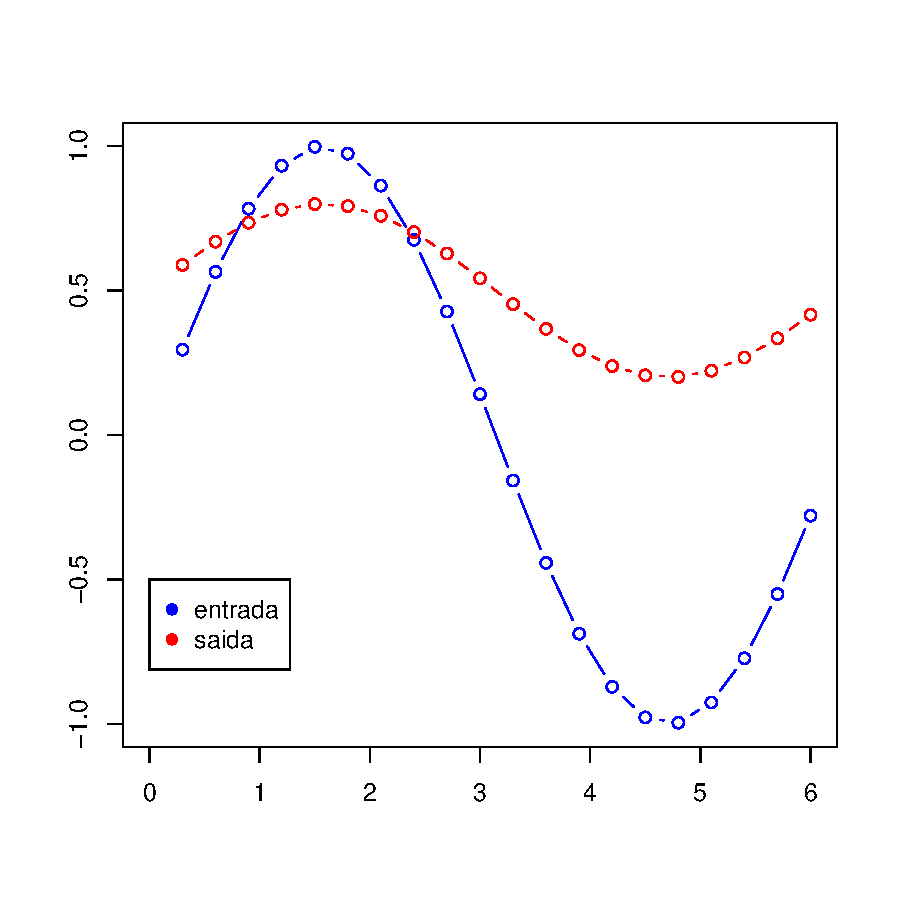
\includegraphics{adaline-001}

\subsection{Treinamento}

O código a seguir utiliza 70\% dos dados da entrada e saída para fazer o treinamento de uma rede neural utilizando Adaline. Os dados são obtidos aleatoriamente.

\begin{Schunk}
\begin{Sinput}
>   source(file='trainadeline.R')
>   n<-as.numeric(dim(x)[1])
>   n_treinamento<-n*0.7
>   seq_treinamento<-sample(n)
>   x_treinamento<-as.matrix(x[seq_treinamento[1:n_treinamento]])
>   y_treinamento<-as.matrix(y[seq_treinamento[1:n_treinamento]])
>   retlist<-trainadeline(x_treinamento,y_treinamento,0.01,0.01,100,1)
>   wt<-as.matrix(retlist[[1]])
>   x_teste<-as.matrix(x[seq_treinamento[(n_treinamento+1):n]])
>   y_teste<-as.matrix(y[seq_treinamento[(n_treinamento+1):n]])
>   y_validacao<-cbind(1,x_teste) %*% wt
\end{Sinput}
\end{Schunk}

\subsection{Cálculo do erro}

O código apresentado abaixo calcula o erro para os dados de testes, 30\% de todos os dados.

\begin{Schunk}
\begin{Sinput}
>   n_teste<-n-n_treinamento
>   erro<-0
>   for(i in 1:n_teste)
+     erro<-erro + (y_teste[i]-y_validacao[i])^2
>   erro<-erro/n_teste
>   erro  
\end{Sinput}
\begin{Soutput}
[1] 0.01419848
\end{Soutput}
\end{Schunk}

\subsection{Gráfico de Comparação}

O código a seguir mostra a comparação entre o $y$ dado com o $y$ previsto pelo modelo:

\begin{Schunk}
\begin{Sinput}
>   y_grafico<-cbind(1,x) %*% wt
>   plot(t,y,type='b',col='gray',ylim=c(-1,1),xlim=c(0,6),xlab='',ylab='')
>   par(new=T)
>   plot(t,y_grafico,type='b',col='green',ylim=c(-1,1),xlim=c(0,6),xlab='',ylab='')
>   legend(0,-0.5,c("original", "previsto"),col=c("gray","green"),pch=16)
\end{Sinput}
\end{Schunk}
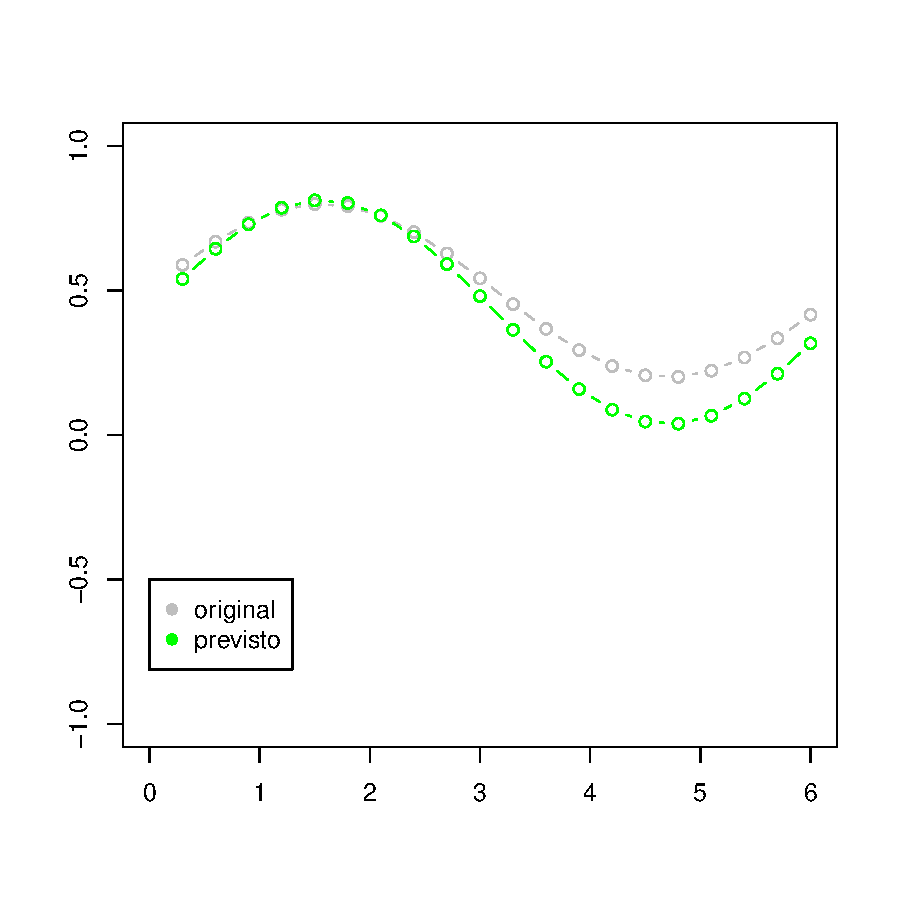
\includegraphics{adaline-echoT}

\subsection{Parâmetros do Modelo}

Os parâmetros obtidos para o modelo foram os seguintes:

\begin{Schunk}
\begin{Sinput}
>   wt
\end{Sinput}
\begin{Soutput}
          [,1]
[1,] 0.4254308
[2,] 0.3877954
\end{Soutput}
\end{Schunk}

\section{Exercício 2}

No segundo exercício, o sinal de entrada é composto por três sinais e a saída é uma mistura desses sinais mais um ganho do tipo: $y = a + b*x_1 + c*x_2 + d*x_3$.

\subsection{Dados de Entrada}

O código a seguir obtém as variáveis $t$, $x$ e $y$ a partir dos arquivos fornecidos. Ao final é plotado o gráfico com os quatro sinais: entradas, $x_1$, $x_2$ e $x_3$ e a saída, $y$, em função de $t$.

\begin{Schunk}
\begin{Sinput}
>   rm(list = ls())
>   t<-as.matrix(read.table('Ex2_t'))
>   x<-as.matrix(read.table('Ex2_x'))
>   y<-as.matrix(read.table('Ex2_y'))
>   x1<-x[,1]
>   x2<-x[,2]
>   x3<-x[,3]
>   par(mfrow=c(2,2))
>   plot(t, x1, type='b', col='red')
>   plot(t, x2, type='b', col='green')
>   plot(t, x3, type='b', col='blue')
>   plot(t, y, type='b', col='orange')
\end{Sinput}
\end{Schunk}
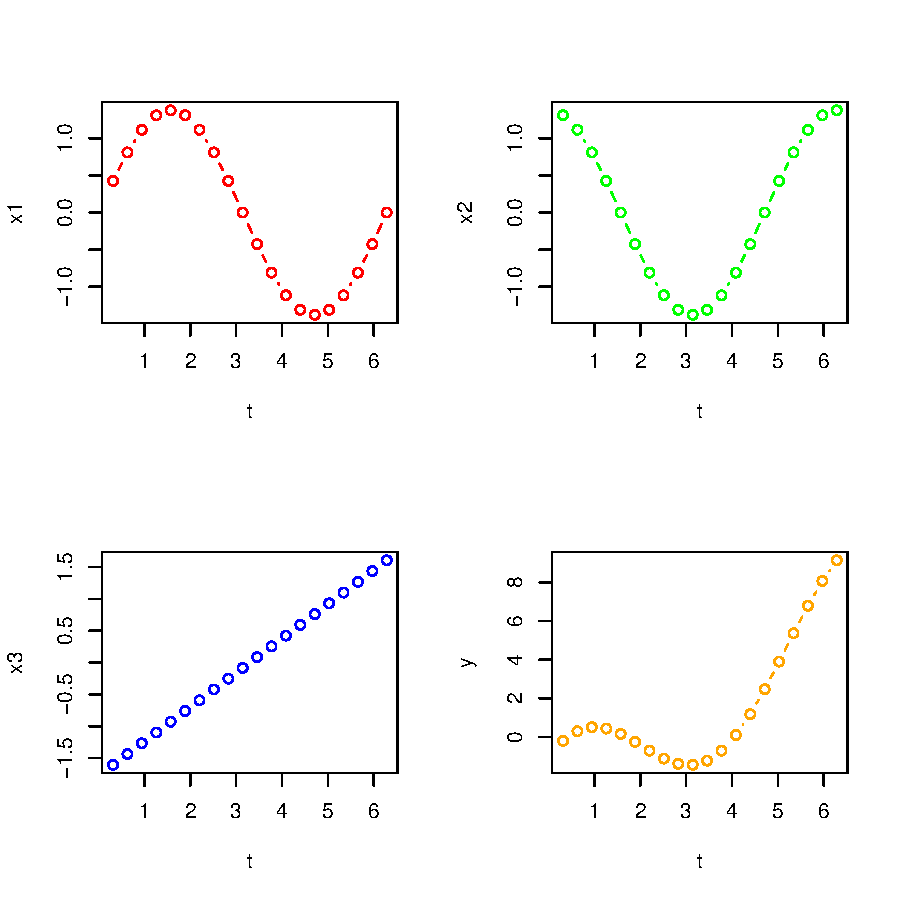
\includegraphics{adaline-006}

\subsection{Treinamento}

O código a seguir utiliza 70\% dos dados da entrada e saída para fazer o treinamento de uma rede neural utilizando Adaline. Os dados são obtidos aleatoriamente.

\begin{Schunk}
\begin{Sinput}
>   source(file='trainadeline.R')
>   n<-as.numeric(dim(t)[1])
>   n_treinamento<-n*0.7
>   seq_treinamento<-sample(n)
>   x1_treinamento<-as.matrix(x1[seq_treinamento[1:n_treinamento]])
>   x2_treinamento<-as.matrix(x2[seq_treinamento[1:n_treinamento]])
>   x3_treinamento<-as.matrix(x3[seq_treinamento[1:n_treinamento]])
>   y_treinamento<-as.matrix(y[seq_treinamento[1:n_treinamento]])
>   x_treinamento<-cbind(x1_treinamento, x2_treinamento, x3_treinamento)
>   retlist<-trainadeline(x_treinamento,y_treinamento,0.01,0.01,100,1)
>   wt<-as.matrix(retlist[[1]])
>   x1_teste<-as.matrix(x1[seq_treinamento[(n_treinamento+1):n]])
>   x2_teste<-as.matrix(x2[seq_treinamento[(n_treinamento+1):n]])
>   x3_teste<-as.matrix(x3[seq_treinamento[(n_treinamento+1):n]])
>   y_teste<-as.matrix(y[seq_treinamento[(n_treinamento+1):n]])
>   y_validacao<-cbind(1,x1_teste,x2_teste,x3_teste) %*% wt
\end{Sinput}
\end{Schunk}

\subsection{Cálculo do erro}

O código apresentado abaixo calcula o erro para os dados de testes, 30\% de todos os dados.

\begin{Schunk}
\begin{Sinput}
>   n_teste<-n-n_treinamento
>   erro<-0
>   for(i in 1:n_teste)
+     erro<-erro + (y_teste[i]-y_validacao[i])^2
>   erro<-erro/n_teste
>   erro  
\end{Sinput}
\begin{Soutput}
[1] 0.005229513
\end{Soutput}
\end{Schunk}

\subsection{Gráfico de Comparação}

O código a seguir mostra a comparação entre o $y$ dado com o $y$ previsto pelo modelo:

\begin{Schunk}
\begin{Sinput}
>   y_grafico<-cbind(1,x1,x2,x3) %*% wt
>   par(mfrow=c(1,1))
>   plot(t,y,type='b',col='gray',ylim=c(-2,10),xlim=c(0,6.5),xlab='',ylab='')
>   par(new=T)
>   plot(t,y_grafico,type='b',col='green',ylim=c(-2,10),xlim=c(0,6.5),xlab='',ylab='')
>   legend(0,6,c("original", "previsto"),col=c("gray","green"),pch=16)
\end{Sinput}
\end{Schunk}
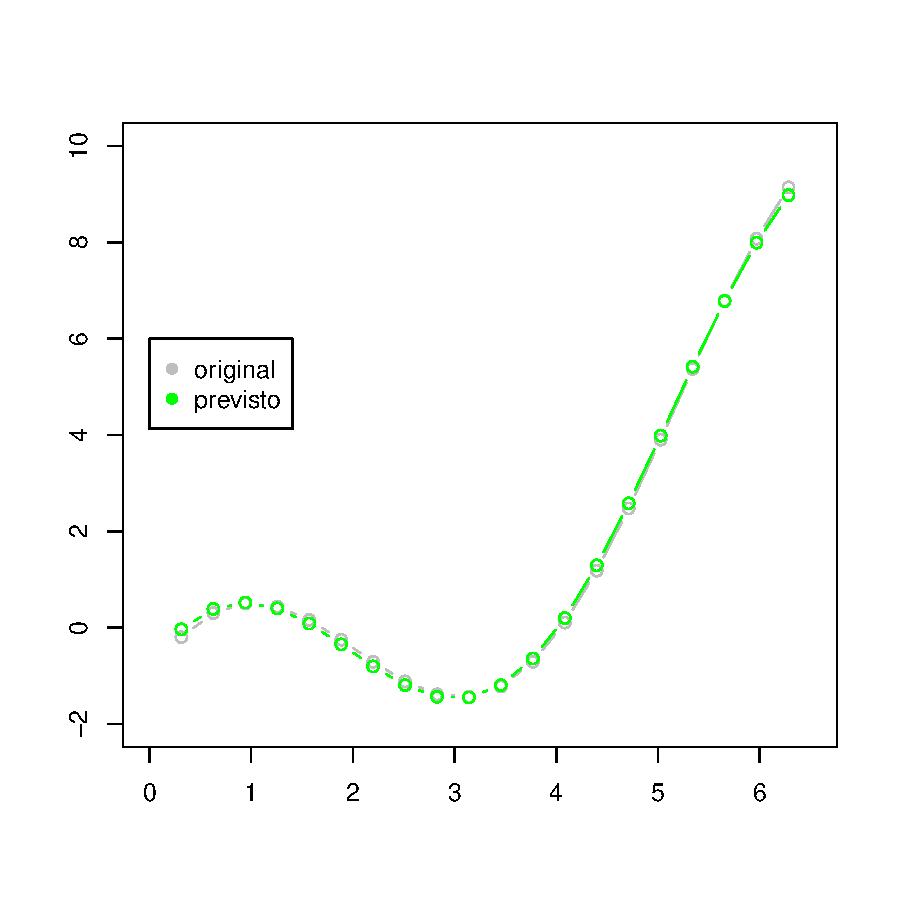
\includegraphics{adaline-009}

\subsection{Parâmetros do Modelo}

Os parâmetros obtidos para o modelo foram os seguintes:

\begin{Schunk}
\begin{Sinput}
>   wt
\end{Sinput}
\begin{Soutput}
          [,1]
[1,] 1.5757983
[2,] 0.8583359
[3,] 2.0192633
[4,] 2.8782880
\end{Soutput}
\end{Schunk}
\end{document}
